\documentclass[12pt,english,letterpaper,article]{memoir}
\usepackage[]{fourier}
\usepackage{amssymb,amsmath}
\usepackage{ifxetex,ifluatex}
\usepackage{fixltx2e} % provides \textsubscript
\ifnum 0\ifxetex 1\fi\ifluatex 1\fi=0 % if pdftex
  \usepackage[T1]{fontenc}
  \usepackage[utf8]{inputenc}
\else % if luatex or xelatex
  \ifxetex
    \usepackage{mathspec}
  \else
    \usepackage{fontspec}
  \fi
  \defaultfontfeatures{Ligatures=TeX,Scale=MatchLowercase}
\fi
% use upquote if available, for straight quotes in verbatim environments
\IfFileExists{upquote.sty}{\usepackage{upquote}}{}
% use microtype if available
\IfFileExists{microtype.sty}{%
\usepackage{microtype}
\UseMicrotypeSet[protrusion]{basicmath} % disable protrusion for tt fonts
}{}
\usepackage[inner=1.5in, outer=1.5in, top=1.5in, bottom=1.75in]{geometry}
\usepackage[unicode=true]{hyperref}
\PassOptionsToPackage{usenames,dvipsnames}{color} % color is loaded by hyperref
\hypersetup{
            pdftitle={ASTRO 250 Final Project},
            pdfauthor={Kolen Cheung},
            pdfkeywords={ASTRO250, Parallel Computing, POLARBEAR, CMB, final project},
            colorlinks=true,
            linkcolor=blue,
            citecolor=blue,
            urlcolor=blue,
            breaklinks=true}
\urlstyle{same}  % don't use monospace font for urls
\ifnum 0\ifxetex 1\fi\ifluatex 1\fi=0 % if pdftex
  \usepackage[shorthands=off,main=english]{babel}
\else
  \usepackage{polyglossia}
  \setmainlanguage[]{english}
\fi
\usepackage{graphicx,grffile}
\makeatletter
\def\maxwidth{\ifdim\Gin@nat@width>\linewidth\linewidth\else\Gin@nat@width\fi}
\def\maxheight{\ifdim\Gin@nat@height>\textheight\textheight\else\Gin@nat@height\fi}
\makeatother
% Scale images if necessary, so that they will not overflow the page
% margins by default, and it is still possible to overwrite the defaults
% using explicit options in \includegraphics[width, height, ...]{}
\setkeys{Gin}{width=\maxwidth,height=\maxheight,keepaspectratio}
\IfFileExists{parskip.sty}{%
\usepackage{parskip}
}{% else
\setlength{\parindent}{0pt}
\setlength{\parskip}{6pt plus 2pt minus 1pt}
}
\setlength{\emergencystretch}{3em}  % prevent overfull lines
\providecommand{\tightlist}{%
  \setlength{\itemsep}{0pt}\setlength{\parskip}{0pt}}
\setcounter{secnumdepth}{5}
% Redefines (sub)paragraphs to behave more like sections
\ifx\paragraph\undefined\else
\let\oldparagraph\paragraph
\renewcommand{\paragraph}[1]{\oldparagraph{#1}\mbox{}}
\fi
\ifx\subparagraph\undefined\else
\let\oldsubparagraph\subparagraph
\renewcommand{\subparagraph}[1]{\oldsubparagraph{#1}\mbox{}}
\fi

% set default figure placement to htbp
\makeatletter
\def\fps@figure{htbp}
\makeatother

\usepackage{siunitx, physics, amsmath}

\title{ASTRO 250 Final Project}
\providecommand{\subtitle}[1]{}
\subtitle{Spring 2017, University of California, Berkeley}
\author{Kolen Cheung}
\date{May  5, 2017}

\begin{document}
\maketitle
\begin{abstract}
Abstract here.
\end{abstract}

{
\hypersetup{linkcolor=blue}
\setcounter{tocdepth}{0}
\tableofcontents
}
\chapter{Introduction}\label{introduction}

Physicists always push the boundary of our understanding of the most
fundamental aspects of the Universe. Some of the fundamental questions
we can ask are what constitute the Universe; how gravity plays a role in
quantum Physics; why neutrino mass are non-zero, how much mass do they
have, and how many numbers of them; and if the current understanding of
the Universe through \(\Lambda\)-CDM model is correct.

Many of such questions can only be answered when we probed at higher and
higher energy scales. For example, the highest energy scale we can
achieve artificially in the state-of-the-art LHC is about
\sim \(\SI{10}{\TeV}\), or \(\SI{10^13}{\eV}\). But we can do only so
much experimentally because of the limit of the size of the equipment we
can build, and it is unlikely for the foreseeable future to create
energy scale as high as the GUT scale at \sim \(\SI{10^16}{\GeV}\), or
\(\SI{10^25}{\eV}\), which will be important for Quantum Gravity.

So instead of relying on human-built machine, one can measure the
primordial signals created by the Universe itself. And the oldest
possible such signal that is observable is the Cosmic Microwave
Background (CMB) Radiation. It is the first light of the Universe when
it was \sim \(\SI{400000}{\yr}\) young, and everything happened between
now and then are imprinted in this signal. Some of the information we
can extracts includes gravitational wave at GUT scale (by B-mode
analysis on the CMB), dark matter, neutrino mass, falsification of
\(\Lambda\)-CDM model, etc.

POLARBEAR, which is one of the pioneer group on the measurement of CMB
polarization in University of California, Berkeley, has conducted about
2 years of observations. One of the major result by POLARBEAR in 2014 is

\begin{quote}
the hypothesis of no B-mode polarization power from gravitational
lensing is rejected at \(97.2\%\) confidence \cite{Collaboration:2014eg}
\end{quote}

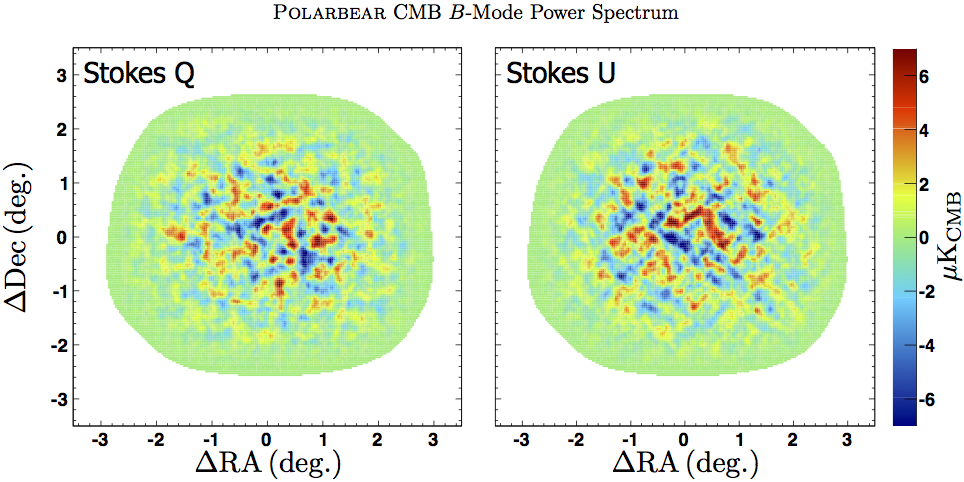
\includegraphics{CMB-B-mode.png}~

But in order to extract more information from the huge amount of data
collected, we need to do a so called high-\(l\) analysis. Previously,
the resolution of the map shown above is made with a lower resolution
than the telescope is capable of. We want to analyze the CMB in full
resolution from the telescope data, which is much more computational
intensive and requires much more scratch disk space.

\chapter{Algorithm}\label{algorithm}

The majority of the algorithms involved are custom-deigned for the
experiments, which relies on existing libraries such as Numpy. On NERSC,
Intel's Distribution of Python (with Anaconda) is used, and therefore
those libraries such as Numpy are built with OpenMP and SIMD support.

Among the custom codes, there are 2 major bottleneck:

\begin{enumerate}
\tightlist
\item
  pseudo-power spectrum (computational intensive),
\item
  weighted averages and statistics (huge intermediate write on scratch
  disks).
\end{enumerate}

The followings layout the plan to solve these 2 problems.

\chapter{Parallelization and
Scalability}\label{parallelization-and-scalability}

Although many functions from different libraries are used, and OpenMP
and SIMD support are built in from the Intel's Distribution of Python,
there are also many custom Python/C code that is custom built, and
unfortunately are all in serial due to historical reasons.

Part of this project is to study the viability of rewriting the code in
Cython instead. Cython is a superset of Python which can be translated
into C/C++ code and compiled. Because of that, we can continue to write
Pythonically when performance is not critical, but in C-style if
performance and critical. Moreover, SIMD optimization and OpenMP are
also supported but limited. Fortunately, since our analysis involve
telescope data, where each hour-long observation are independent, and
each channels within an observation are also independent for most of the
analysis, parallelizing the code within the Cython language is doable in
all the performance critical loops in my study. There is a vectorization
that can only be achieved by \texttt{\#pragma\ ivdep} in C and
unfortunately not supported in Cython, but is not performance critical.
In fact, OpenMP parallelization is so easy to use in Cython, that most
effort of OpenMP parallelization is not spent on whether it is
parallelizable but whether if it is worth the OpenMP overhead because
the algorithm might be I/O bounded.

\section{Optimizations and
Improvements}\label{optimizations-and-improvements}

Here we will focus on the 2 limiting factors that makes the current
analysis very expensive, and a proposal on solving these 2 problems. And
lastly, the time and space cost is estimated.

\chapter{Computational Hotspot}\label{computational-hotspot}

In the current pipeline, the computation cost is estimated to be:

\begin{itemize}
\tightlist
\item
  \(700\) simulation and \(1\) real data
\item
  \(14\) splits for null test
\item
  \(90 \min\) per spectra
\item
  \(3\) spectra each
\item
  Cori Haswell charge factor: \(80 \hr\) per node
\item
  \(16\) processes per node due to RAM limit
\end{itemize}

So the total amount of NERSC hours needed are \sim \(220,000\) NERSC
hours.

One of the most computational intensive part of the pipeline is the
apodization mask in the pseudo-power spectrum, which basically smoothen
the transition on the boundary. The old algorithm is \(O(n^3)\) and
relies on Numpy's functions and because of the limited choices of
functions, the algorithm is going through unnecessary steps and is very
slow. I proposed an algorithm that is \(O(n)\), based on a boundary
tracing algorithm. Although this algorithm is very hard to parallelize,
it scales as \(O(n)\) which shows its advantage when we are doing a full
resolution analysis as \(n\) becomes very large.

In addition, I expect speed-up from Cythonization including SIMD
vectorization and OpenMP multi-threading. From OpenMP, I estimated we
would get about a 4-fold improvement, because in our current pipeline we
only start 16 processes on Cori's Haswell nodes due to RAM limit and
therefore wasting half numbers of idle cores, and since our pipeline are
mostly IO bounded, I expect another 2-fold from multi-threading. From
SIMD, I conservatively estimate a factor of 2 improvement, because of
vectorization efficiency, some loops cannot be vectorized, and some are
already done in the Numpy functions. I expect a 4-fold improvement from
Cythonization based on preliminary test due to the inefficiency of using
Numpy in Python. And conservatively, we divide it by a factor of 2 to
account for possible overestimation. So the total speed-up factor is
estimated to be 16.

So to conclude, if all optimization scheme laid out above is used, the
total number of NERSC hours needed for this analysis would be
\sim \(14,000 \hr\).

However, cythonization is a lengthy process. To account for the fact
that we want to perform this analysis as soon as possible and therefore
we might not be able to fully cythonize our application, we
conservatively estimated we need \(100,000\) NERSC hours, including
profiling and debugging cost.

\chapter{Disk Space Hotspot}\label{disk-space-hotspot}

In the current pipeline, a lot of intermediate files are written. In the
1st stage of the pipeline, each of \(4237\) files will have one output,
and then a 2nd stage process will load them to co-add them together
(calculate a weighted average as well as statistics). So the total
intermediate disk space required is:

\begin{itemize}
\tightlist
\item
  \(12.3 \MB\) per observation
\item
  \(4237\) observations
\item
  ``null factor'' --- the extra disk space required for null test:
  \(6.67 \pm 0.01\)
\item
  700 simulation and 1 real data
\end{itemize}

with a total of \(244\TB\).

In ideal situation, one would use an MPI reduce to avoid all the
intermediate files. However, the legacy code base is too spaghetti-like
for such kind of refactoring. My proposal is for each independent
process, rather then writing a new output files, it will open the
previous one, co-add, and then close the files. So the number of
intermediate files no longer proportional to the total number of input
\(4237\), but the total number of process, which is much less:

\begin{itemize}
\tightlist
\item
  original size: \(244\TB\)
\item
  Intermediate disk size: \(20\TB\) from Cori's scratch
\item
  \(4237\) inputs
\item
  \(16\) process per node
\end{itemize}

so we can start at most \(21\) nodes at a time. And from the above
computational time estimate, the wall clock time required will be
\sim \(8 \hr\) in the best case senario, and \(57 \hr\) in the
conservative estimate. Since the maximum wall-clock time that can be
requested is \(36 \hr\) when \(21\) nodes is used, the jobs might be
needed to be split in 2.

Because of the huge amount of IO, Cori's burst buffer seems to be best
fit for this task.

\end{document}
